\documentclass[a4paper,openright,11pt]{report}

%
% Times New Roman font.
%
\usefont{T1}{ptm}{m}{n}
\selectfont


% Packages a utilizar e respetivos parâmetros.
\usepackage{indentfirst}
\usepackage{inputenc}
\usepackage{enumitem}
\usepackage[portuguese]{babel}
\usepackage{graphicx}
\usepackage{float}
\usepackage{url}

\makeatletter
\let\NAT@parse\undefined
\makeatother
\usepackage{hyperref}

\addto{\captionsenglish}{\renewcommand{\bibname}{References}}
% Definições das dimensões das páginas
\setlength{\textheight}{24.00cm}
\setlength{\textwidth}{15.50cm}
\setlength{\topmargin}{0.35cm}
\setlength{\headheight}{0cm}
\setlength{\headsep}{0cm}
\setlength{\oddsidemargin}{0.25cm}
\setlength{\evensidemargin}{0.25cm}

\newcommand{\comment}[1]{}
%
% Times New Roman font.
%
\usefont{T1}{ptm}{m}{n}
\selectfont

%
%title
%
\title{%
  \vspace{-55mm}
  \begin{minipage}[l]{150mm}
    \resizebox{50mm}{!}{
\includegraphics{./figures/logo_isel.png}}
  \end{minipage}\\
  \vspace{20mm}
  \bfseries{Corporate Collaboration \par Relatório Final}
}

%
%authors
%
\author{%
  \begin{tabular}{lll}
      & 45365 David Fidalgo \\
  \\
    & 45366 Pedro Santos \\
   
  \\
    & 44865 Valdemar Antunes \\
    
  \end{tabular}
} 

%
% date
%
\date{%
\vspace{30mm}
\begin{center}
  \begin{tabular}{ccc}
    & {Orientadores:} \\
    & Paula Graça, ISEL, paula.graca@isel.pt \\
    & Diogo Pacheco, Do iT Lean, diogo.pacheco@doitlean.com\\
  \end{tabular}\\
\end{center}
\vspace{20mm}
Relatório final realizado no âmbito de Projecto e Seminário,\\
do curso de licenciatura em Engenharia Informática e de Computadores\\
Semestre de Verão 2019/2020
\vspace{10mm}\\
24 de Julho de 2020}

\begin{document}
\thispagestyle{empty}
\maketitle

\tableofcontents{}\label{index:chapters}
\listoffigures{}\label{index:figures}
\newpage

\chapter{Introdução}\label{sec:intro}

\section{Enquadramento}\label{sec:enquadramento}
O mercado de hoje, cada vez mais tecnológico, exigente e desafiador, impõe um ritmo às empresas que, para
além de gerirem os seus principais processos de negócio, estas têm também uma dinâmica significativa de
atividades internas para as ajudar no seu crescimento e competitividade. Em particular, as empresas do setor
das tecnologias de informação, mantêm atividades internas tais como participação em feiras de emprego,
partilha de conhecimento através de apresentações informais, desenvolvimento de componentes de software,
ofertas de formação, atividades lúdicas, entre muitas outras. Para isso, tem que existir uma coordenação de
recursos que nem sempre é fácil, dada a sua alocação aos projetos em curso. Contudo, se existir um
planeamento atempado gerido através de uma plataforma de colaboração, o processo pode ser agilizado,
permitindo não só o registo e divulgação das necessidades internas, bem como a aceitação de candidaturas por
parte dos colaboradores mais interessados na sua realização.

\section{Objetivos}\label{sec:objectivos}
A aplicação proposta visa a implementação de uma plataforma colaborativa para agilizar a resposta a necessidades internas das empresas, nomeadamente a
organização de eventos, partilha de conhecimento, ofertas formativas, entre outras. 
Os objetivos que a plataforma visa atingir consistem na divulgação de comunicados para a comunidade da empresa;
no contexto de um evento, incluem a partilha de localização, 
gestão de recursos, registo de presenças, registo de candidaturas e gestão das mesmas; 
a calendarização de eventos e, por último, um sistema de notificações.

\chapter{Formulação do Problema}\label{chapter:formulacaoDoProblema}

O desenvolvimento da plataforma \textit{Corporate Collaboration} pretende atingir certos requisitos, de forma a poder enquadrá-la no mercado 
atual. 


\section{Estado da Arte}\label{sec:estadoDaArte}
As plataformas de colaboração existentes no mercado atual tais como a \textit{Microsoft SharePoint} ou a \textit{BaseCamp} apresentam um elevado nível de complexidade, 
incluindo ferramentas como calendários partilhados, partilha de ficheiros, mensagens instantâneas, armazenamento na \textit{cloud}, video-conferência, entre outros. 
A aplicação desenvolvida neste âmbito não procura igualar todas as funcionalidades das plataformas já existentes, 
mas sim, agilizar a dinâmica de atividades internas que ocorrem diariamente nas empresas. 
Visa, essencialmente, facilitar a procura de pessoas para cumprir certas necessidades que existam no âmbito das atividades internas da empresa, 
necessidades estas que permitem definir uma tarefa que tem de ser realizada ou um evento que será organizado no contexto da dinâmica interna da empresa. 
Estas necessidades são auxiliadas por recursos que permitem gerir candidaturas e participantes das mesmas, 
assim como apresentar informações sobre alojamento, refeições, transporte e localização, se for caso disso.

\section{Análise de Requisitos}\label{sec:requisitos}

As funcionalidades principais da plataforma \textit{Corporate Collaboration} estão representadas na figura~\ref{fig:uc:generalActions}

\begin{figure}[H]
    \centering
    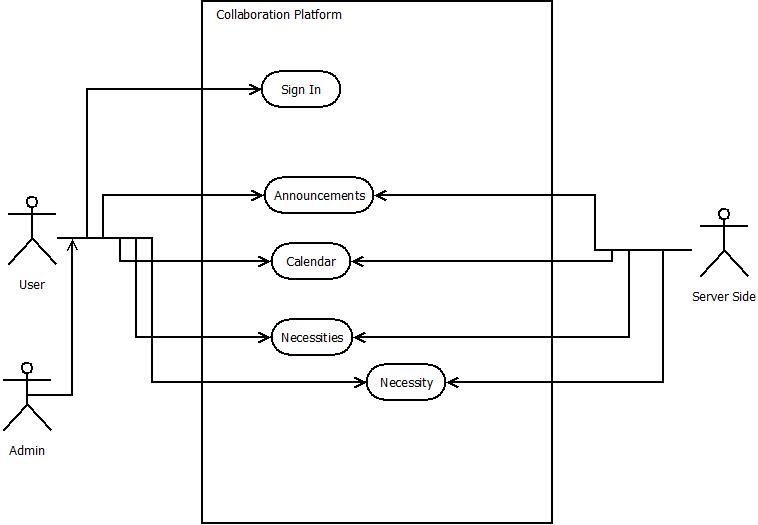
\includegraphics[scale=0.6]{figures/General Actions.jpeg}
    \caption{\textit{Use Case} --- Ações gerais.}\label{fig:uc:generalActions}
\end{figure}

\subsection{Registo e Autenticação}\label{subsec:login}
Para desenvolver a funcionalidade de registo e autenticação na plataforma de colaboração é necessário existir uma tabela 
na base de dados que guarde as credenciais e informação básica de cada utilizador, nomeadamente 
o \textit{email}, \textit{password}, \textit{username}, primeiro e último nome. 
Esta tabela tanto serve para efeitos de registo de um utilizador, como para verificação posterior da sua autenticação. 
Os utilizadores não necessitam de fazer registo na aplicação, visto que nesta plataforma é suposto utilizarem 
as mesmas credenciais atribuidas pela empresa, para e-mail e autenticação nas outras aplicações internas.

Relativamente ao ecrã de \textit{Login} ilustrado na figura~\ref{fig:uc:login}, este suporta:

\begin{itemize}
    \item Duas caixas de texto onde o utilizador introduz o seu e-mail e password.
    \item Um botão identificado como \textit{Login} que desencadeia o processo de verificação das credencias introduzidas.
\end{itemize}

\begin{figure}[H]
    \centering
    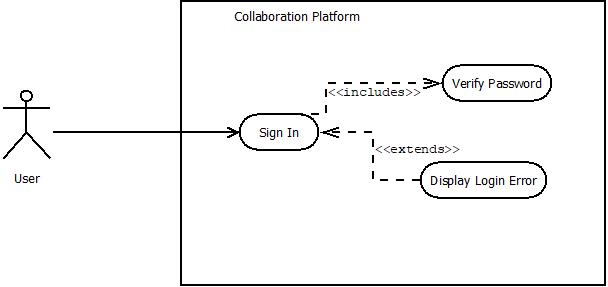
\includegraphics[scale=0.6]{figures/Login Use Case.jpeg}
    \caption{\textit{Use Case} --- \textit{Login}.}\label{fig:uc:login}
\end{figure}

O utilizador com permissões de administrador tem acesso ao \textit{back-office} onde pode criar ou remover categorias.

\subsection{\textit{Home Page --- Dashboard}}\label{subsec:dashboard}

Após o \textit{login} na aplicação o utilizador será redirecionado para um novo ecrã que irá conter um \textit{dashboard} com o intuito de organizar e 
apresentar a informação de uma forma apelativa. As necessidades a que o utilizador se candidatou serão apresentadas neste \textit{dashboard}. 
O mesmo irá conter também uma secção com estatística relativa ao número de necessidades que existem em cada categoria. 
A seleção de uma das categorias na estatística redirecionará o utilizador para o ecrã das necessidades, 
apresentando a lista das mesmas com o filtro correspondente à categoria selecionada. 

\subsection{Registo das necessidades internas da empresa, gestão de candidaturas, notificações e integração com o google maps}\label{subsec:necessitiesCandidatesNotificationsGoogleMaps}

A funcionalidade de registo de necessidades internas da empresa estão organizadas em categorias de modo a facilitar a navegação do utilizador pelas mesmas.

\begin{figure}[H]
    \centering
    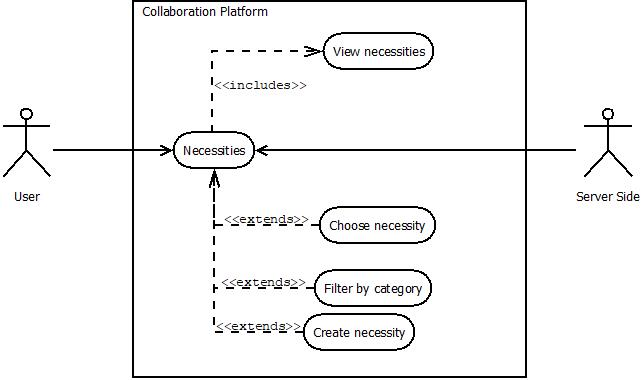
\includegraphics[scale=0.6]{figures/Necessities.jpeg}
    \caption{\textit{Use Case} --- Necessidades.}\label{fig:uc:necessities}
\end{figure}

Para isso, é fundamental que exista um ecrã que apresente todas as necessidades da empresa. 
Um utilizador, caso queira registar uma necessidade, irá escolher a categoria que melhor se adequa à mesma. 
Caso não exista, este, se tiver permissões de admin, poderá criar uma categoria nova no \textit{back-office} da aplicação. 
Neste ecrã será possível filtrar as necessidades pela sua categoria e pelo seu grau de urgência.

\begin{figure}[H]
    \centering
    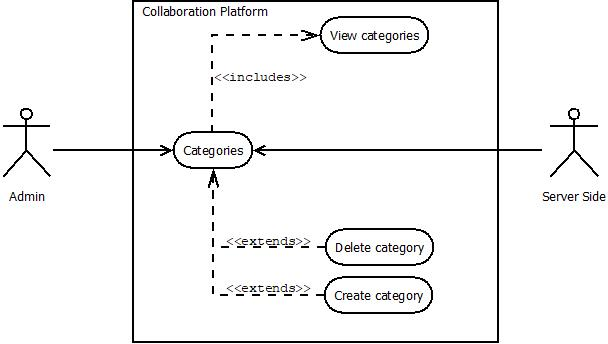
\includegraphics[scale=0.6]{figures/Categories use case.jpeg}
    \caption{\textit{Use Case} --- Categorias.}\label{fig:uc:categories}
\end{figure}

Posto isto, definimos um conjunto de filtros que podem ser conjugados de modo a permitir um melhor agrupamento e organização das necessidades. O primeiro consiste na filtragem por categorias, como por exemplo \textit{Brown Bags}, 
\textit{Qualification Offers}, \textit{Software Components Development} ou \textit{Planning of Events}. 
Foi ainda definido um segundo filtro que poderá tomar os valores \textit{High}, \textit{Medium} ou \textit{Low}, 
correspondentes ao grau de prioridade com que as necessidades foram criadas. 
A seleção dos filtros irá levar a uma atualização da lista para conter apenas necessidades que se enquadrem nessa mesma seleção. 
Este ecrã apresenta ainda um botão que servirá para criar uma nova necessidade, criação esta acessível a todos os utilizadores autenticados, 
que decorrerá num novo ecrã e que terá como opção (obrigatória) de criação os filtros a qual associar a nova necessidade. 
Em cada necessidade existe a possibilidade de associar recursos com informações sobre alojamento, refeições, localização do evento ou transporte para o local onde a mesma se irá realizar. Todos os recursos, com exceção do recurso transporte, têm associado um mapa do \textit{Google Maps} onde os utilizadores podem fornecer informações sobre localização.
Ao clicar numa necessidade, será apresentado um novo ecrã com os detalhes da mesma, com os recursos associados e também a possibilidade do utilizador se candidatar como colaborador ou participante da necessidade, dependendo da fase em que a mesma se encontra. O autor da necessidade irá receber a notificação de que existe um novo candidato, 
dando-lhe a opção de após carregar na notificação ser redirecionado para o ecrã de detalhe da necessidade onde pode observar os candidatos. 
Ao criar uma necessidade o autor tem a possibilidade de escolher se todas as candidaturas à necessidade em causa são aceites automaticamente ou se o próprio escolhe os candidatos com base na descrição dada pelos mesmos.  
O candidato irá receber uma notificação nos casos em que a necessidade for fechada/cancelada, e quando a sua candidatura for aceite/recusada. 
Terá também a possibilidade de ver quem já se candidatou á necessidade criada pelo próprio no ecrã de detalhe na parte dos participantes, estando candidatos a colaboradores separados de candidatos a participantes. 
O ecrã que permite mostrar as notificações associadas a cada utilizador é acedido ao carregar no ícone em forma de sino presente na barra da aplicação. Este ícone tem um pequeno contador associado que indica o número de notificações pendentes que cada utilizador tem e, quando pressionado, é apresentado o ecrã das notificações onde as mesmas são apresentadas na forma de uma lista. 

\begin{figure}[H]
    \centering
    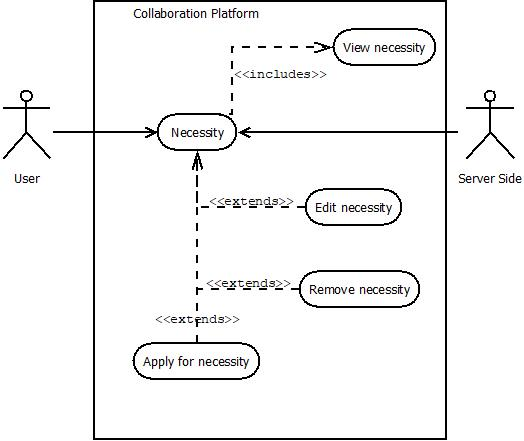
\includegraphics[scale=0.6]{figures/Necessity.jpeg}
    \caption{\textit{Use Case} --- Necessidade.}\label{fig:uc:necessity}
\end{figure}

Exemplificando, para organizar eventos ou feiras de emprego, o utilizador seleciona a categoria \textit{Planning of events}.

Se por outro lado, tivermos o objetivo de realizar apresentações informais de partilha de conhecimento o utilizador seleciona a categoria \textit{Brown Bags}. 
Todos os utilizadores devidamente autenticados podem candidatar-se para assistir a uma dada apresentação ou para a orientar. 
No contexto da necessidade é definida uma linha temporal que consiste numa primeira fase de candidaturas para escolha do orientador 
(ou orientadores) que irão conduzir a apresentação, seguida de uma segunda fase de candidaturas para utilizadores que queiram assistir à apresentação. 
O autor de uma apresentação, no ecrã de detalhe da mesma, terá acesso a quem se candidatou para a orientar, podendo escolher um ou mais orientadores 
com base na descrição apresentada pelos mesmos. 
Numa segunda fase após a escolha do(s) mesmo(s), o autor pode ver os utilizadores que se 
candidataram à necessidade no seu ecrã de detalhe e todos os utilizadores autenticados podem ver quem foi aceite/vai ao evento.

%%%%%%%%%%%%%%%%%%%%%%%%%%%%%%%%%%%%%%%%%%%%%%%%%%%%%%%%%%%%%%%%%%%%%%%%%%%%%%%%%%%%%%%%%%%%%%%%%%%%%%%%%%
\comment{
    A categoria \textit{Make a Post} tem como objetivo a criação de um post numa rede social ou blog. 
    O utilizador ao filtrar esta categoria ser-lhe-á apresentado a lista dos posts. 
    O utilizador ao carregar num post navegará para um novo ecrã que apresentará os detalhes do mesmo. 
    Os detalhes apresentados para um post já publicado incluem uma breve descrição, um link para o post e a pessoa que o realizou. 
    Os detalhes para um post não publicado incluem a possibilidade de o utilizador se candidatar para o realizar, assim como uma breve descrição.

    Com o objetivo de possibilitar ofertas de formação dentro da empresa, foi definida a categoria \textit{Qualification Offers}. 
    Esta categoria apresenta uma dinâmica semelhante à categoria \textit{Informal Presentations}, visto que ambas procuram a partilha de 
    conhecimento por parte de um ou mais oradores, definidos numa primeira instância, seguida de uma segunda fase em que os utilizadores 
    poderão manifestar a sua intenção em participar. 
    O principal fator que distingue estas duas categorias é a duração da atividade: 
    uma oferta de formação decorrerá ao longo de várias sessões satisfazendo um número total de horas apresentado na descrição da necessidade, 
    ao contrário de uma apresentação informal que é um acontecimento único de duração na ordem dos minutos. 
    Posto isto, a dinâmica apresentada nesta categoria quanto ao ecrã de detalhes e metodologia será semelhante à da categoria \textit{Brown Bags}.

    A categoria \textit{Software Components Development} tem como objetivo propor projetos e procurar participantes para os mesmos, no âmbito de desenvolvimento de software. 
    Ao ser selecionada uma proposta será apresentado um novo ecrã com a sua descrição, detalhes e com um botão que permitirá ao utilizador 
    candidatar-se para integrar o projeto.

    Com o objetivo de proporcionar oportunidades de progressão na carreira de forma espontânea, por exemplo, 
    haver uma vaga para uma posição de tech lead num novo projeto, e os seniors interessados poderem candidatar-se a esta posição. 
    O utilizador após selecionar a categoria \textit{Opportunities for Career Progression} serão apresentadas todas as necessidades correspondentes, sob a forma de uma lista.

    A categoria \textit{Off-work Activities} permite a criação de necessidades com o intuito de realizar atividades lúdicas.
    Um autor desta atividade tem de endereçar os meios de transporte bem como se existe almoço e/ou jantar e as ementas para a respetiva refeição. 
    A funcionalidade de candidaturas nesta categoria funciona de forma a que cada utilizador manifeste a sua vontade em participar no evento.
    Antes do \textit{deadline} desta atividade o utilizador tem de confirmar a sua participação.
}
%%%%%%%%%%%%%%%%%%%%%%%%%%%%%%%%%%%%%%%%%%%%%%%%%%%%%%%%%%%%%%%%%%%%%%%%%%%%%%%%%%%%%%%%%%%%%%%%%%%%%%%%%%
\subsection{Divulgação e calendarização das necessidades}

Com o objetivo de divulgar e calendarizar as necessidades internas da empresa, a barra de navegação da aplicação terá um botão que, quando carregado, 
redireciona o utilizador para um ecrã que apresenta um calendário com o qual ele poderá interagir. 
Neste calendário são apresentados todos os eventos organizados, na sua respetiva data, e existe a possibilidade de filtrar os eventos em que o mesmo participará. 
Após a seleção de um dia no calendário, são apresentados os eventos, dando a possibilidade ao utilizador de ver os detalhes individuais após carregar num deles, 
num novo ecrã.

\begin{figure}[H]
    \centering
    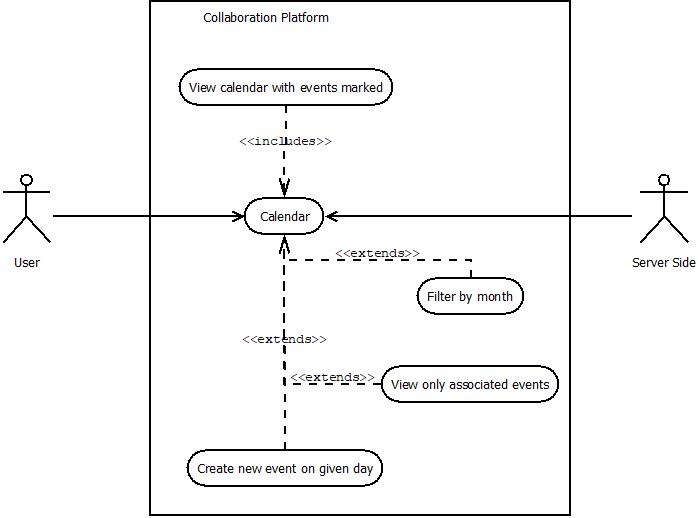
\includegraphics[scale=0.6]{figures/Calendar use case.jpeg}
    \caption{\textit{Use case} --- Calendário.}\label{fig:uc:calendar}
\end{figure}

Para ser possível divulgar as necessidades da empresa de forma uniforme por todos os seus colaboradores, a barra de navegação da aplicação apresentará 
um botão denominado \textit{Announcements} que, quando carregado, abre um ecrã  (figura~\ref{fig:uc:announcements}) que contém os comunicados sobre a forma de uma lista. 
Sempre que for emitido um novo comunicado todos os utililizadores recebem uma notificação com o título do mesmo e, ao carregar nessa notificação, são redirecionados para os detalhes do comunicado. 
Estes comunicados foram criados por um utilizador com permissões de administrador, sendo visíveis por todos os que estejam autenticados.

\begin{figure}[H]
    \centering
    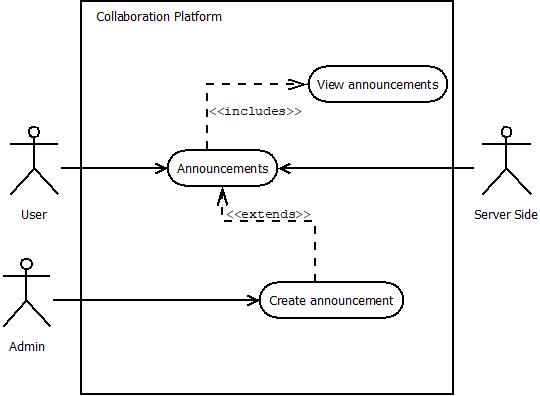
\includegraphics[scale=0.6]{figures/Announcements use case.jpeg}
    \caption{\textit{Use case} --- Announcements.}\label{fig:uc:announcements}
\end{figure}

\section{Plataforma OutSystems}\label{sec:plataformaOutSystems}

A escolha da plataforma \textit{OutSystems~\cite{outsystems}}, para a implementação deste projeto baseia-se essencialmente no facto da mesma ser \textit{low-code},
apresentando vários benefícios essenciais para um projeto de curto prazo como o apresentado. A rapidez
com que é possível produzir peças de \textit{software}, as funcionalidades \textit{user-friendly} como \textit{drag and drop} e 
interfaces de utilizador pré-feitas e a possibilidade de produzir aplicações automaticamente através de
um simples clique, são elementos essenciais que levaram à escolha desta plataforma. 
Cada \textit{endpoint} da aplicação está associado a um ecrã com o qual o utilizador interage, havendo uma navegabilidade entre ecrãs que permitindo, assim,
 que o utilizador visite os diferentes \textit{endpoints} da aplicação.
A criação e utilização de \textit{blocks} é uma das funcionalidades altamente vantajosas que a plataforma \textit{OutSystems~\cite{outsystems}} apresenta, 
visto que permite a reutilização deste componente ao longo da \textit{User Interface --- UI}.
A construção da aplicação torna-se bastante rentável, em termos de tempo e facilidade do desenvolvimento, 
através da conjugação de conceitos como \textit{Widgets}, \textit{Screens} e \textit{Blocks} no domínio da  \textit{UI} 
e de conceitos como \textit{Server Actions} (ações executadas do lado do servidor), \textit{Client Actions} (ações executadas do lado do cliente) 
e \textit{Aggregates} (ação com o propósito de aceder à base de dados para retornar informações persistentes na mesma).
Também é disponibilizado pela \textit{OutSystems~\cite{outsystems}}, um \textit{eSpace} por \textit{module} que contém elementos essenciais 
ao desenvolvimento, como os enunciados anteriormente.
A base de dados está alojada numa \textit{cloud}, onde são guardadas todas as entidades dos vários módulos.


\chapter{Descrição do problema}\label{chapter:description}

O desenvolvimento de uma plataforma colaborativa apresenta diversos desafios ao nível da sua arquitetura, 
do modelo de dados a construir e das decisões de implementação ao longo do seu desenvolvimento. 
Neste capítulo irá ser abordado as decisões tomadas no desenvolvimento do projeto, tendo em conta a plataforma \textit{OutSystems~\cite{outsystems}}. 
Irá ser feita uma descrição mais detalhada da solução adotada, acompanhada por um diagrama de blocos, que permite esquematizar a mesma.


\section{Diagrama de blocos da solução}\label{sec:diagram}
A figura~\ref{fig:diagram} apresenta o diagrama de blocos da plataforma \textit{Corporate Collaboration}. 

\begin{figure}[H]
  \centering
  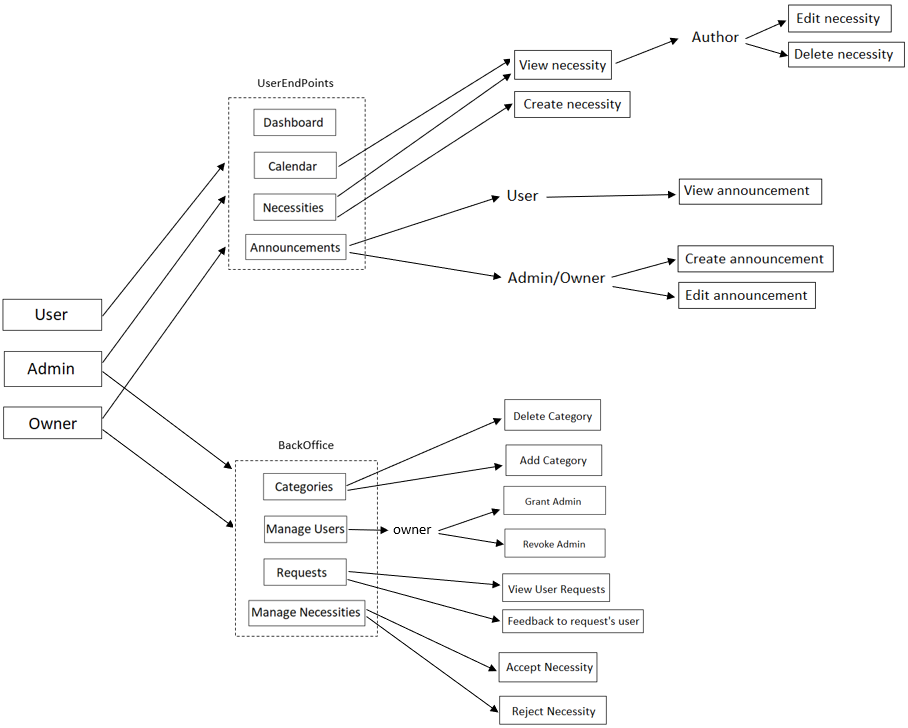
\includegraphics[scale=0.4]{figures/Diagrama de blocos.png}
  \caption{Diagrama de blocos da aplicação}\label{fig:diagram}
\end{figure}

\newpage

\section{Arquitetura}\label{sec:arquitechture}

\subsection{Plataforma \textit{OutSystems}}\label{sec:OutSystemsArch}

A arquitetura desta plataforma pode ser observada na figura~\ref{fig:outsystemsArch}. 
O principal componente da plataforma é o Platform Server que permite que as aplicações 
desenvolvidas sejam geradas, optimizadas, compiladas e publicadas. 

\begin{figure}[H]
  \centering
  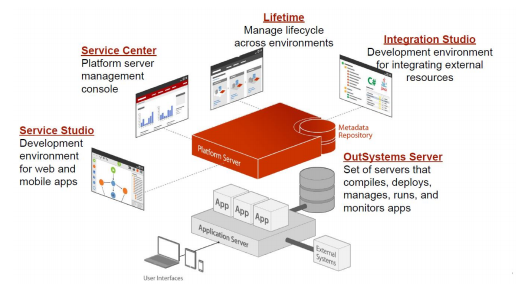
\includegraphics[]{figures/Architecture.png}
  \caption{Arquitetura da plataforma \textit{OutSystems~\cite{outsystems}}}\label{fig:outsystemsArch}
\end{figure}

Este componente usa os seguintes serviços: 
\begin{enumerate}
  \item \textit{Code Generator} --- Usa a aplicação modelada no \textit{Service Studio} e gera o código necessário usando tecnologias standard (como \textit{.NET, SQL Server, HTML,} etc.) para a criação de uma aplicação optimizada e segura.
  \item \textit{Deployment Services} --- Publica o código que foi previamente gerado no servidor, assegurando que a aplicação é instalada consistentemente em cada front-end da infraestrutura.
  \item \textit{Application Services} --- Gere as aplicações durante o runtime, através da execução de \textit{batches} agendados e serviços de \textit{logging} assíncronos que permitem que sejam armazenados eventos como erros, inspeções e métricas de desempenho.
\end{enumerate}

\newpage

\subsection{Arquitetura 4 Layer Canvas}\label{sec:4lc}

Para desenharmos a arquitetura da nossa solução, seguimos a metodologia da plataforma \textit{OutSystems~\cite{outsystems}}, a \textit{4 Layer Canvas} apresentado na figura~\ref{fig:4lc}.

\begin{figure}[H]
  \centering 
  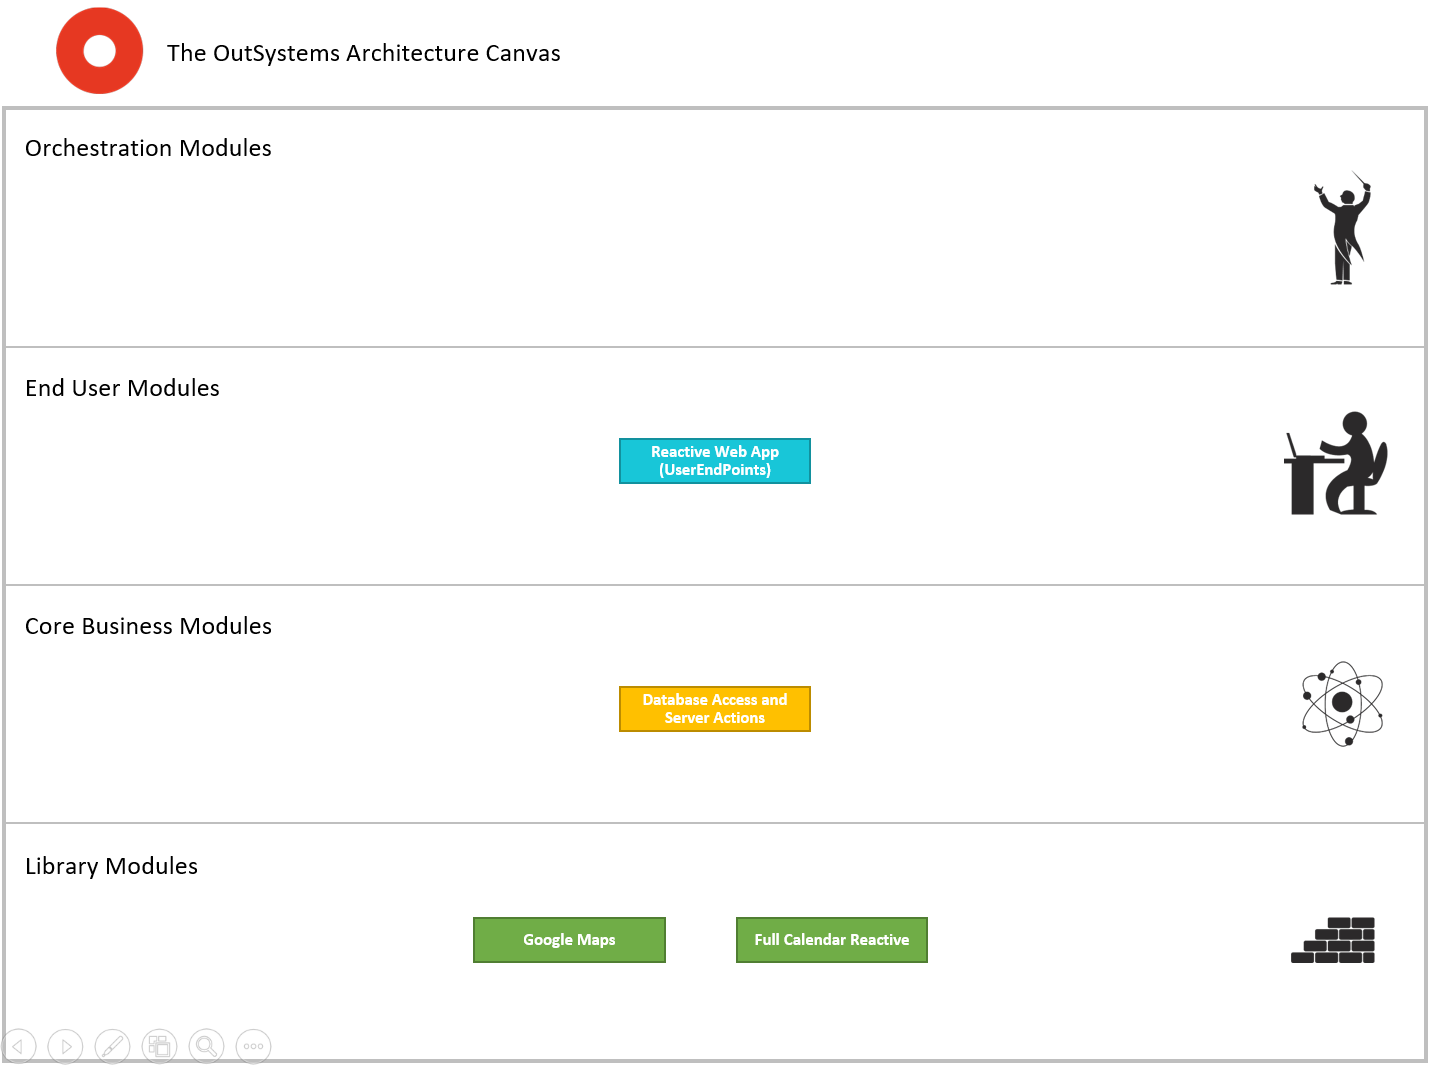
\includegraphics[scale=0.5]{figures/4LayerCanvas.png}
  \caption{4 \textit{Layer Canvas}}\label{fig:4lc}
\end{figure}

Esta metodologia propõe que se estruture as várias funcionalidades da aplicação por quatro camadas, sendo estas, começando por baixo: 

\begin{itemize}
    \item \textit{Library Layer} --- Aqui devem constar os módulos que são transversais ao domínio do problema, tais como: temas, bibliotecas, etc. 
    \item \textit{Core Layer} --- Módulos referentes à lógica de negócio, modelo de dados e \textit{server actions}. 
    \item \textit{End User Layer} --- Nesta camada é tratada toda a parte de interface e experiência do utilizador, fazendo uso das camadas anteriores. 
    \item \textit{Orchestration Layer} --- Camada que coordena a comunicação entre várias aplicações. 
\end{itemize}

É importante verificar que, apesar da metodologia apresentar quatro camadas, 
a nossa arquitetura apenas faz uso das primeiras três devido ao nosso projeto consistir em apenas uma aplicação reactive, 
e não havendo necessidade de coordenar interações com outras aplicações na camada de orquestração. 
Posto isto, a nossa aplicação assenta sobre cinco módulos, representados pela figura~\ref{fig:4lc}.

Começando pela \textit{Library Layer} verificamos que são utilizados os módulos relativos à integração da aplicação 
com o \textit{Google Maps} e com o \textit{Full Calendar Reactive}. De seguida temos a \textit{ Core Layer}, 
onde definimos as entidades de domínio e suas operações. Por fim a \textit{ End User Layer} onde são definidos 
os ecrãs e a lógica de cliente. 

\section{Modelo de Dados}\label{subsec:ModeloDados}

O conceito predominante no modelo de dados, (figura~\ref{fig:modeloDados}), é o de necessidade, representado pela tabela \textit{Necessity}.

\begin{figure}[H]
  \centering 
  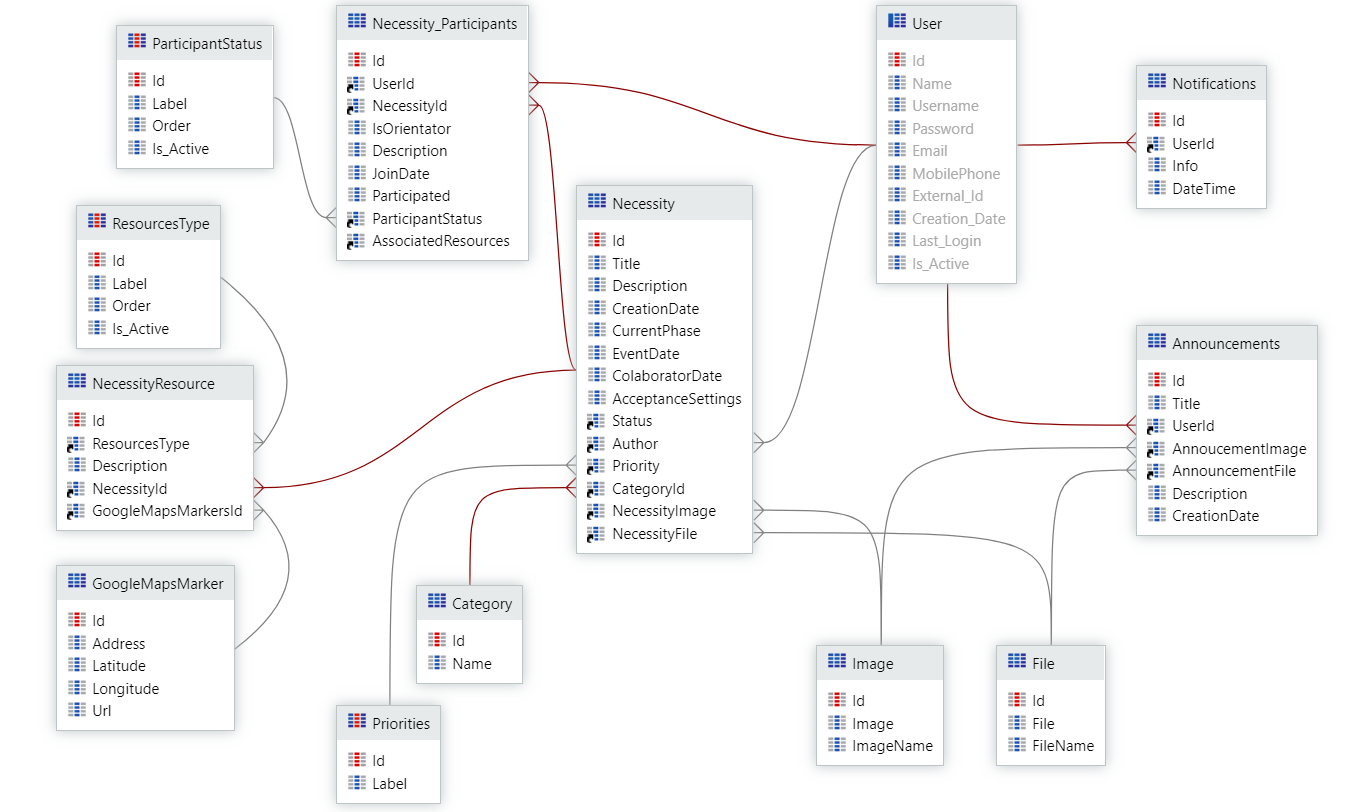
\includegraphics[scale=0.4]{figures/DataModel.png}
  \caption{Modelo de dados}\label{fig:modeloDados}
\end{figure}

 
Uma necessidade é caracterizada por diversos elementos dos quais destacamos o \textit{Status} que referencia uma tabela estática (\textit{NecessityStatus}) que contém os valores possíveis do estado da necessidade, 
podendo ter os valores \"Closed\", \"Active\" ou \"Archived\". A \textit{CurrentPhase} que indica a fase de candidaturas atual, 
podendo ser para orientadores ou participantes, a \textit{ColaboratorDate} que representa a data limite das candidaturas 
à posição de orientador e ainda \textit{AcceptanceSettings} que indica se para a necessidade em causa são aceites todos os participantes ou se existe uma filtragem por parte do autor. 
As tabelas \textit{NecessityImage} e \textit{NecessityFile} existem para o propósito de guardar ficheiros, 
aliviando a quantidade de dados guardada em cada tuplo \textit{Necessity}, 
seguindo também as boas práticas da plataforma \textit{OutSystems~\cite{outsystems}}. 
A entidade estática \textit{Priorities} contém os valores possíveis das prioridades que cada necessidade pode ter.
Associado ao conceito de necessidade está o de recurso, que tem como objetivo acrescentar informação à necessidade de uma forma flexível. 
Para suportar este conceito foi definida a entidade estática \textit{ResourcesType} cujos valores representam os tipos de recursos que um utilizador pode, facultativamente, acrescentar à necessidade, consistindo em acomodação, restaurante e menus de refeições, localização do evento ou transporte. 
A representação de um recurso no modelo de dados traduz-se na entidade \textit{NecessityResource} que guarda informações de cada recurso como o seu tipo (referência à tabela  \textit{ResourcesType}), a sua descrição, o id da necessidade a que o mesmo pertence e, como todos os recursos à exceção do relativo ao transporte têm um mapa do \textit{Google Maps} associado
, o último atributo da tabela \textit{NecessityResource} é um id do marcador do mapa associado ao recurso.
Com o objetivo de guardar informação sobre os participantes de uma necessidade, é definida a entidade \texttt{\textit{Necessity\char`_Participants}} que 
contempla o identificador da mesma, o identificador do utilizador, a descrição associada à candidatura, 
se esta candidatura é para posição de orientador ou de participante, a data da candidatura, se o utilizador participou na necessidade, qual o estado da candidatura e os recursos associados a este participante. 
Um utilizador pode ser um participante, um autor ou um orientador da necessidade. 
Os comunicados feitos na plataforma são suportados pela entidade \textit{Announcements}. As notificações apresentadas na plataforma são suportadas pela entidade \textit{Notifications} em que cada notificação está associada a um utilizador através do seu id, o seu conteúdo é guardado no atributo \textit{Info} e a hora da emissão da notificação no atributo \textit{DateTime}. 
Um utilizador pode ainda ter o cargo de administrador, cujos privilégios incluem editar as categorias representadas pela entidade \textit{Category}.

\section{Implementação}\label{sec:implementacao}

\subsection{Autenticação}\label{subsec:implementacao:login}

Para realizar a autenticação de um utilizador, este introduz as suas credenciais nos respetivos \textit{input fields} e clica no botão \textit{Login}.
Se as credenciais introduzidas não corresponderem às de nenhum utilizador na base de dados, será apresentada uma mensagem de erro.
Um utilizador só terá acesso a outros ecrãs se tiver autenticado, caso contrário será redirecionado para este ecrã, figura~\ref{fig:LoginScreen}.

\begin{figure}[H]
  \centering 
  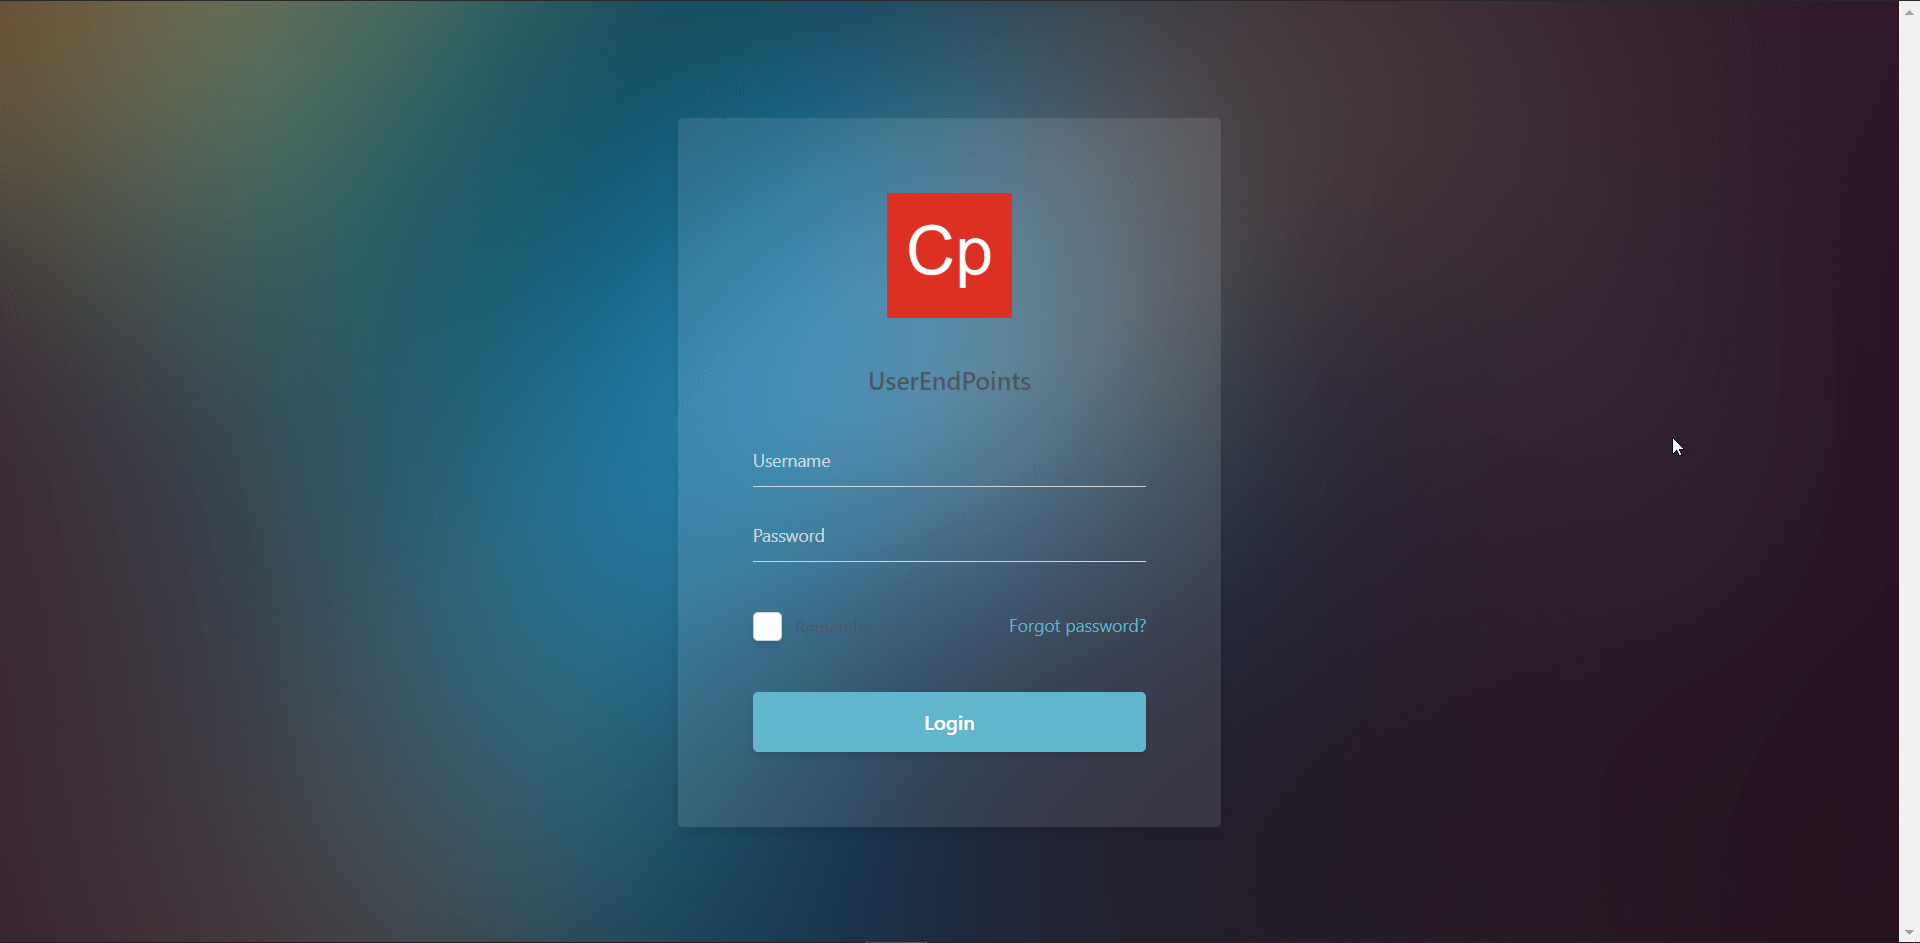
\includegraphics[scale=0.35]{figures/LoginScreen.png}
  \caption{Ecrã de autenticação}\label{fig:LoginScreen}
\end{figure}

\subsection{\textit{Back-office}}\label{subsec:implementacao:back-office}

O \textit{back-office} da \textit{Collaboration Platform} tem como principal motivação a manutenção da mesma e o acesso a funcionalidades que requerem permissões superiores, nomeadamente de \textit{admin} ou de \textit{owner}.
Posto isto, o \textit{back-office} é implementado num novo módulo e apresenta quatro ecrãs distintos. 
No ecrã \textit{Necessities} os utilizadores com acesso ao \textit{back-office} têm a possibilidade de verificar as necessidades criadas pela comunidade da empresa, podendo aceitá-las ou eliminá-las. 
O ecrã \textit{Categories} tem como objetivo a criação e remoção de categorias. 
No ecrã \textit{ManageUsers} é possível ver todos os utilizadores da plataforma separados entre utilizadores comuns e utilizadores com permissões mais elevadas.
Deste modo, existe a possibilidade de alterar as permissões associadas a um utilizador, concedendo-lhe permissões superiores ou removendo. 
Com o intuito de ver as mensagens criadas pela comunidade da empresa, o ecrã \textit{UserMessages} apresenta-as sobre a forma de uma lista e possibilita que cada utilizador sinalize uma mensagem que esteja por resolver como \textit{"resolved"} se aceitar/cumprir o conteúdo da mensagem ou como \textit{"rejected"} se não for o caso.  



\subsection{\textit{Dashboard}}\label{subsec:implementacao:dashboard}

A um utilizador autenticado é apresentado o ecrã da \textit{dashboard} figura~\ref{fig:Dashboard}, quando inicia a aplicação.
O mesmo apresenta quatro \textit{widgets} que apresentam informação sobre o número de utilizadores que estão \textit{logged in} e o número de necessidades abertas com as suas respetivas prioridades (\textit{high, medium, low}).
Este ecrã apresenta também um gráfico com informação sobre as categorias existentes e a distribuição do número de necessidades criadas em cada uma das mesmas.
A seleção de uma categoria do gráfico promove a navegação para o ecrã das necessidades,  apresentando a lista das mesmas que pertencem à categoria selecionada.
Para cada uma das prioridades que as necessidades podem ter, é apresentado um \textit{ranking} dos utilizadores que mais criaram necessidades, com a respetiva prioridade.

\begin{figure}[H]
  \centering 
  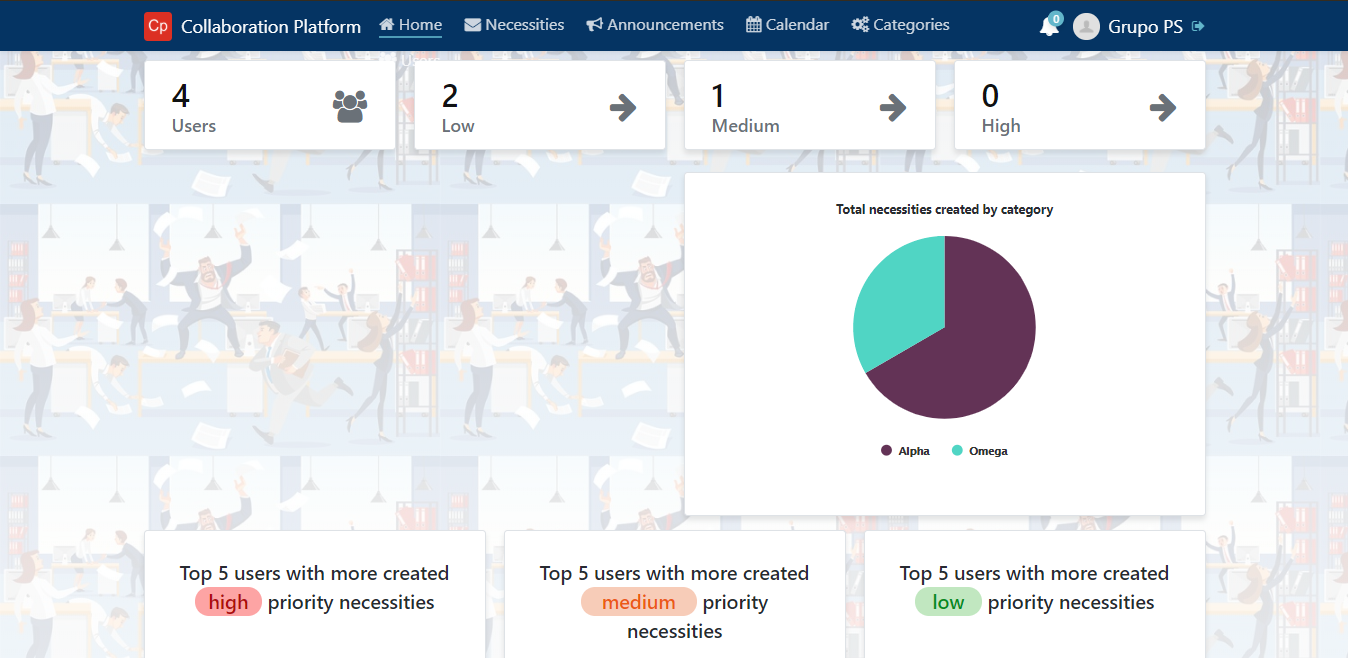
\includegraphics[scale=0.4]{figures/Dashboard.png}
  \caption{\textit{Dashboard}}\label{fig:Dashboard}
\end{figure}


\subsection{Criação e edição de categorias}\label{subsec:implementacao:categories}

Um utilizador com permissões de \textit{admin} tem a possibilidade de aceder ao ecrã \textit{Categories} e de criar ou eliminar categorias. 
É apresentado um \textit{widget} tabela com todas as categorias existentes e um botão delete que permite eliminar as selecionadas.
O processo de criação de uma nova categoria é feito carregando no botão create e inserindo o nome da nova categoria no \textit{popup} que aparece no ecrã, seguido do botão \textit{save}.


\subsection{Visualização de necessidades}\label{subsec:implementacao:necessities}
O utilizador ao carregar no botão \textit{Necessities} presente na barra da aplicação, será redirecionado para o ecrã responsável pela apresentação das necessidades demonstrado na figura~\ref{fig:NecessitiesScreen}. 
O intuito do mesmo consiste na apresentação das necessidades criadas pela comunidade empresarial, sendo possível aplicar filtros e/ou pesquisar pelo título de uma necessidade de modo a que sejam apresentadas apenas as necessidades alvo.
As necessidades são apresentadas num \textit{widget} tabela, cujas colunas apresentam informação relevante como título, categoria, prioridade, estado, data de criação e data em que a necessidade irá decorrer. Sempre que o utilizador pretender criar uma nova necessidade, apenas tem que carregar no botão \textit{Create Necessity} e será redirecionado para um novo ecrã, onde poderá completar a criação.
A seleção do título de uma necessidade promove a navegação para o ecrã dos detalhes da mesma.
A barra de pesquisa permite que o utilizador procure uma necessidade pelo seu título.
Os filtros aplicáveis são apresentados em dois \textit{dropdowns}, um para permitir a escolha de qual a prioridade e outro para seleção da(s) categoria(s).
Sempre que exista uma mudança na seleção de algum dos \textit{widgets} de filtragem de necessidades ou uma introdução de texto na barra de pesquisa, a tabela é atualizada para apresentar apenas aquelas que verifiquem as características alvo. 
As informações de cada uma das necessidades, das categorias existentes e das prioridades são obtidas comunicando com o servidor através de \textit{Aggregates}. 
Os \textit{Aggregates} são \textit{querys} optimizadas à base de dados de modo a retornar informação de forma eficiente e apresentá-la nos \textit{widgets} do ecrã.

\begin{figure}[H]
  \centering 
  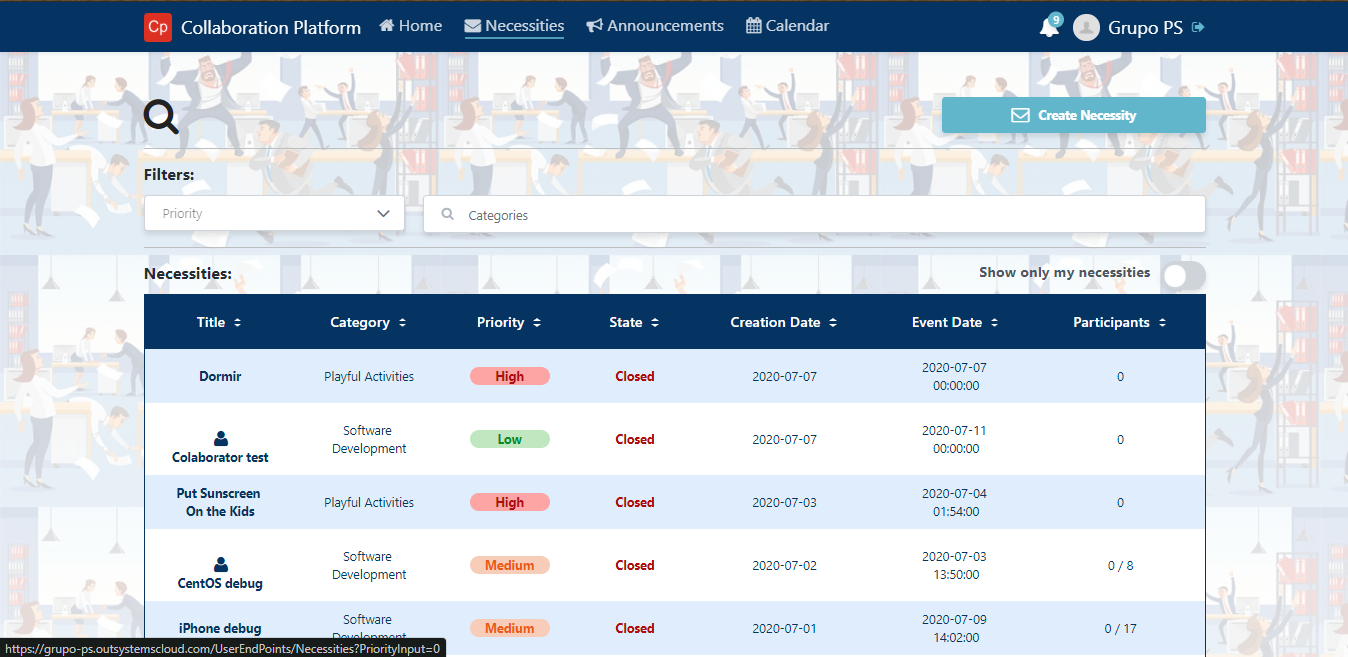
\includegraphics[scale=0.3]{figures/NecessitiesGeneralScreen.png}
  \caption{Ecrã das necessidades.}\label{fig:NecessitiesScreen}
\end{figure}



\subsection{Visualização de necessidades num calendário}\label{subsec:implementacao:calendarNecessitiesView}

O utilizador ao carregar no botão \textit{Calendar} presente na barra da aplicação, será redirecionado para o ecrã, apresentado na figura~\ref{fig:CalendarScreen} responsável por mostrar, num calendário, todas as necessidades existentes organizadas por datas. 
O objetivo deste ecrã é apresentar de uma forma mais organizada e estruturada todas as necessidades criadas pela empresa, sendo possível filtrá-las. 
Para preencher o calendário, para cada necessidade, é criado um objeto \textit{Event} com a sua informação. 
Cada evento estará representado no calendário com uma cor diferente de forma a distinguir entre necessidades criadas pelo utilizador, necessidades associadas, nomeadamente uma inscrição, e necessidades criadas por outros utlizadores.
Se o utilizador carregar num evento, este é redirecionado para o seu ecrã de detalhe. 
É possível filtrar eventos pela sua categoria, através de um popover menu que contém todas as categorias existentes. 
Caso seja selecionada uma categoria, são removidos todos os eventos presentes no calendário, e de seguida, renderizado com os novos eventos filtrados.

\begin{figure}[H]
  \centering 
  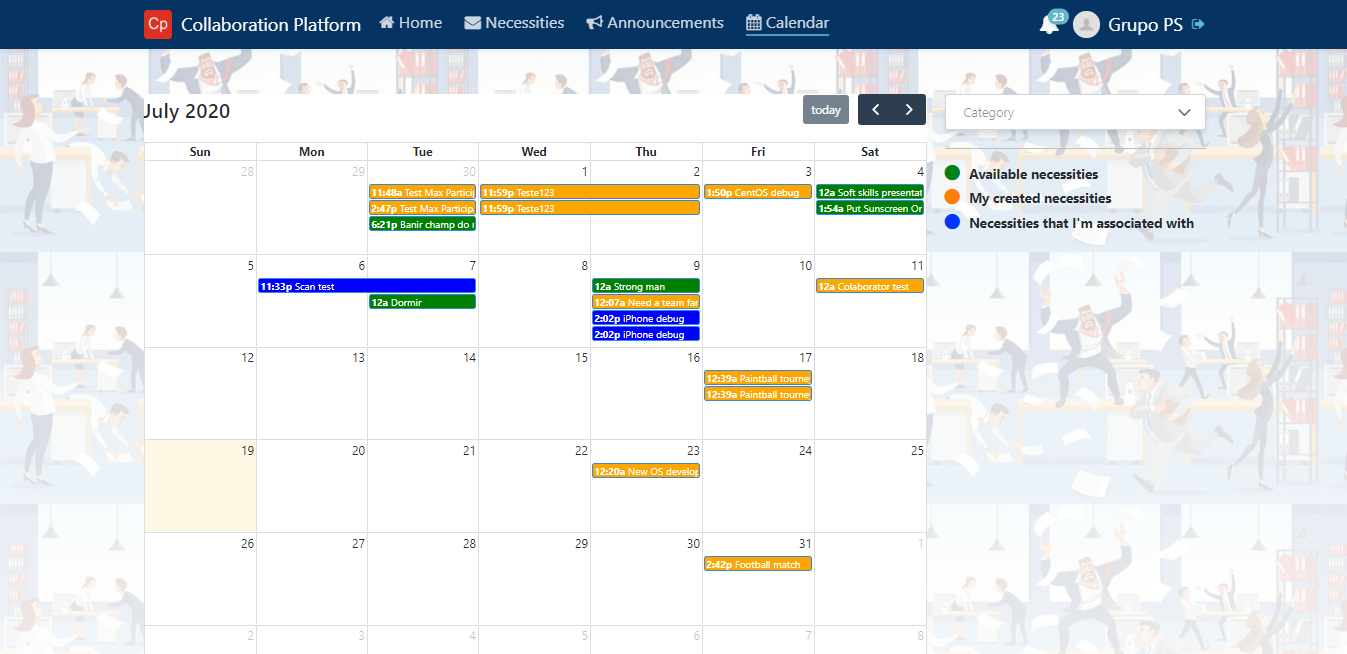
\includegraphics[scale=0.4]{figures/Calendar.png}
  \caption{Ecrã do calendário.}\label{fig:CalendarScreen}
\end{figure}

\subsection{Criação e edição de necessidades}\label{subsec:implementacao:necessityCreation}

O ecrã \textit{NecessityCreation} (figura~\ref{fig:necessityCreation1} e~\ref{fig:necessityCreation2}) é utilizado para criar, editar, remover ou ver os detalhes de uma necessidade.
No momento da criação de uma necessidade os \textit{widgets} presentes neste ecrã permitem que o utilizador indique o título, a descrição, a categoria a qual associar a necessidade, a sua prioridade, 
se existe filtragem de participantes ou todas as candidaturas são aceites, uma imagem e um ficheiro para serem associados à necessidade, a data em que a mesma irá decorrer, se é necessário colaborador(es) e a data limite para a(s) sua(s) candidatura(s).

\begin{figure}[H]
  \centering 
  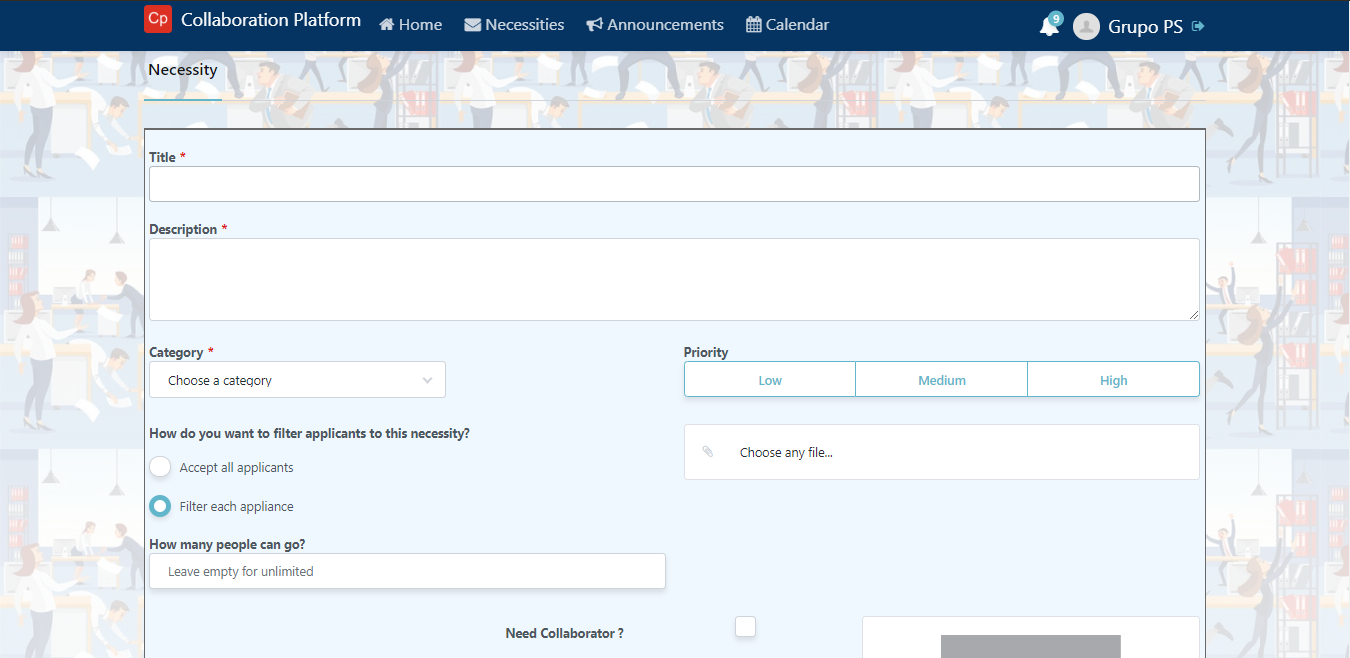
\includegraphics[scale=0.4]{figures/NecessityCreation1.png}
  \caption{Ecrã \textit{Necessity Creation} --- Criação parte 1}\label{fig:necessityCreation1}
\end{figure}



\begin{figure}[H]
  \centering 
  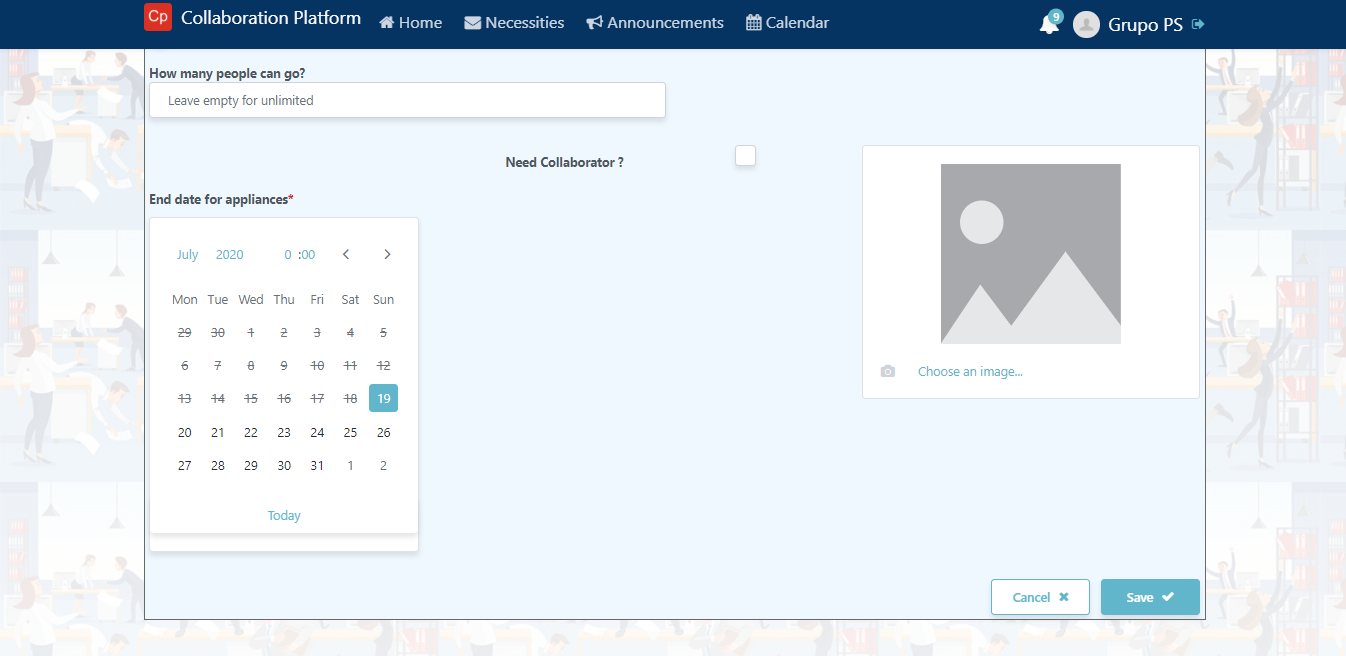
\includegraphics[scale=0.3]{figures/NecessityCreation2.png}
  \caption{Ecrã \textit{Necessity Creation} --- Criação parte 2}\label{fig:necessityCreation2}
\end{figure}


Ao pressionar o botão presente no final do ecrã com a legenda \textit{Save}, tanto num cenário de edição como de criação, 
são guardadas as informações presentes nos \textit{widgets} e é desencadeada uma \textit{client action} que posteriormente cria uma ligação ao servidor através da chamada a uma \textit{server action} para modificar a base de dados com uma nova necessidade ou alterando uma necessidade pré-existente.

Se o utilizador desejar editar ou remover uma necessidade, só o poderá fazer se for o autor desta e, no caso de a editar, o ecrã (figura~\ref{fig:NecessityCreationWithResourcesAndParticipants}) apresentará os campos já preenchidos com os dados atuais da necessidade e a possibilidade de os alterar livremente.

\begin{figure}[H]
  \centering 
  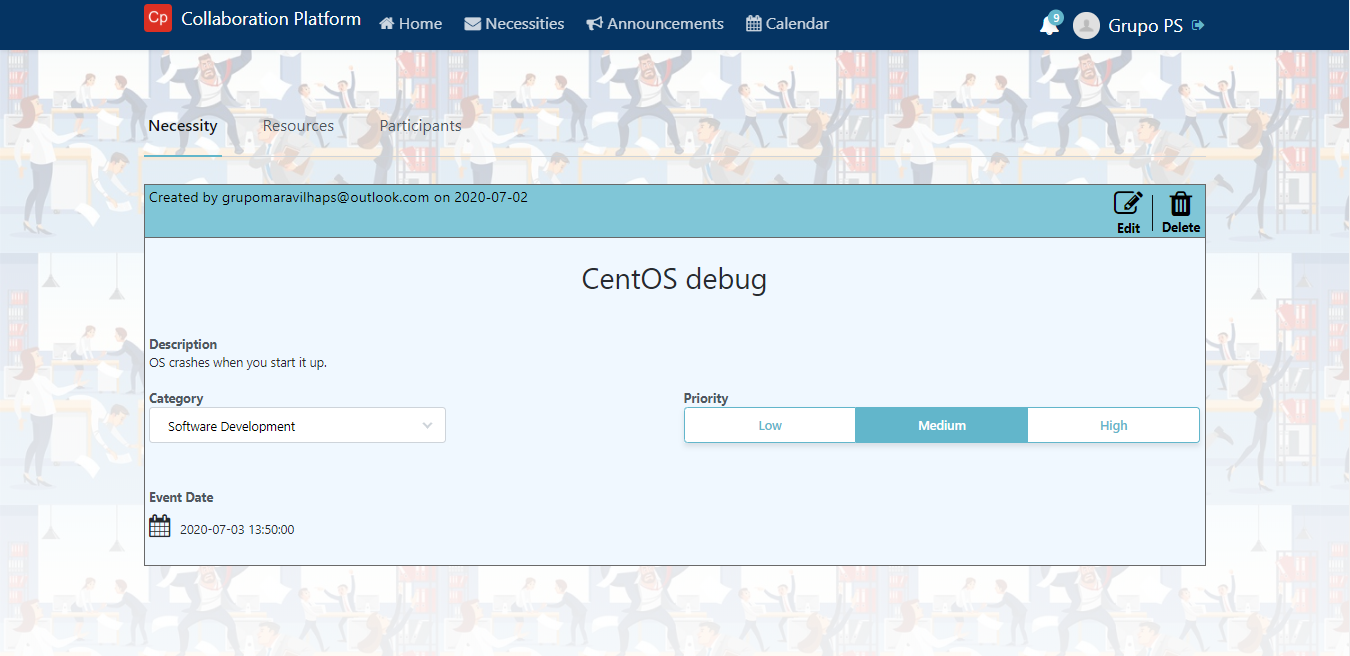
\includegraphics[scale=0.4]{figures/NecessityCreationWithResourcesAndParticipants.png}
  \caption{Ecrã \textit{Necessity Creation} --- Aba de detalhe da necessidade.}\label{fig:NecessityCreationWithResourcesAndParticipants}
\end{figure}


É também neste ecrã (figura~\ref{fig:Resources1}) que o utilizador poderá consultar os recursos associados através da navegação até à tab \textit{Resources} e se for o autor da necessidade pode adicionar novos recursos. 
Todos os recursos com exceção do recurso transporte têm um \textit{block} que contém um mapa do \textit{Google Maps} através do qual o utilizador pode colocar um marker para dar a conhecer a localização associada ao recurso. 
A integração do \textit{Google Maps} (figura~\ref{fig:Resources2}) na plataforma é realizada através da comunicação com a API do \textit{Google Maps}~\cite{google maps api}. Para criar um novo mapa é necessário criar um objeto do tipo \textit{google.maps.Map} que recebe na sua construção o elemento html onde o mapa será inserido. 
Toda a dinâmica de interação com o mapa é gerida pela API através de eventos que são desencadeados com o toque no mesmo. 

\begin{figure}[H]
  \centering 
  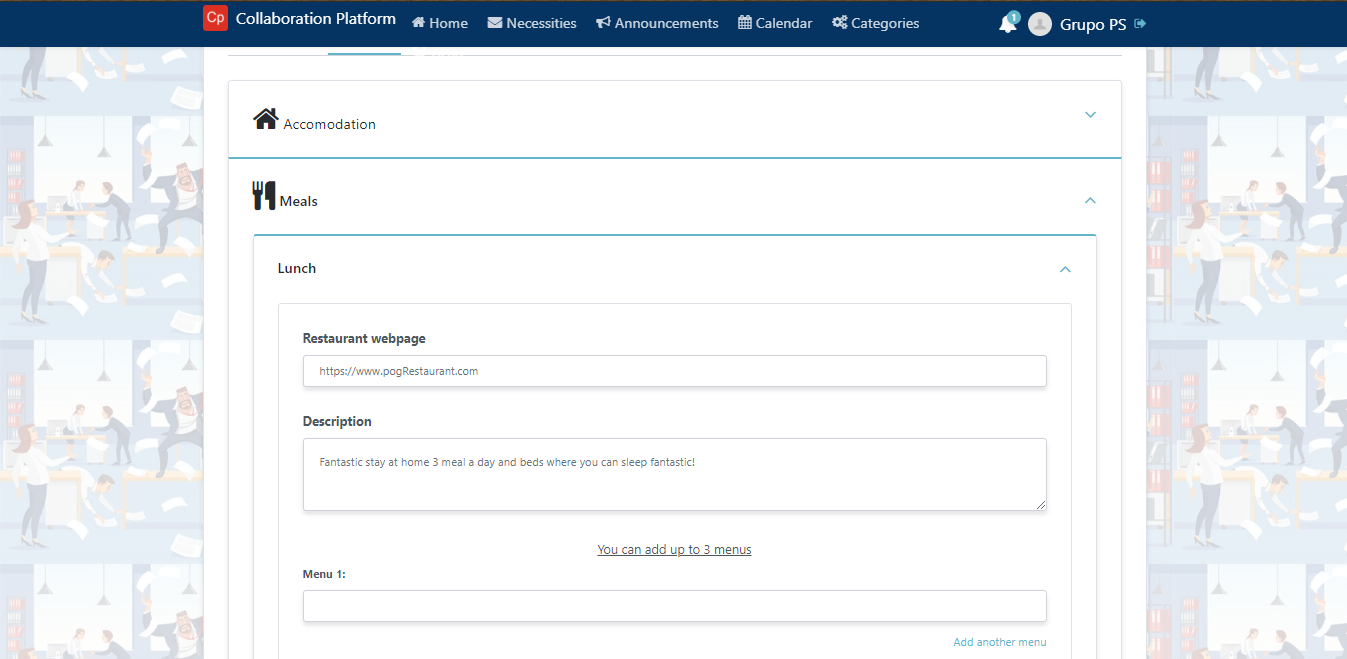
\includegraphics[scale=0.4]{figures/Resources1.png}
  \caption{Ecrã \textit{Necessity Creation} --- Aba de recursos parte 1.}\label{fig:Resources1}
\end{figure}



\begin{figure}[H]
  \centering 
  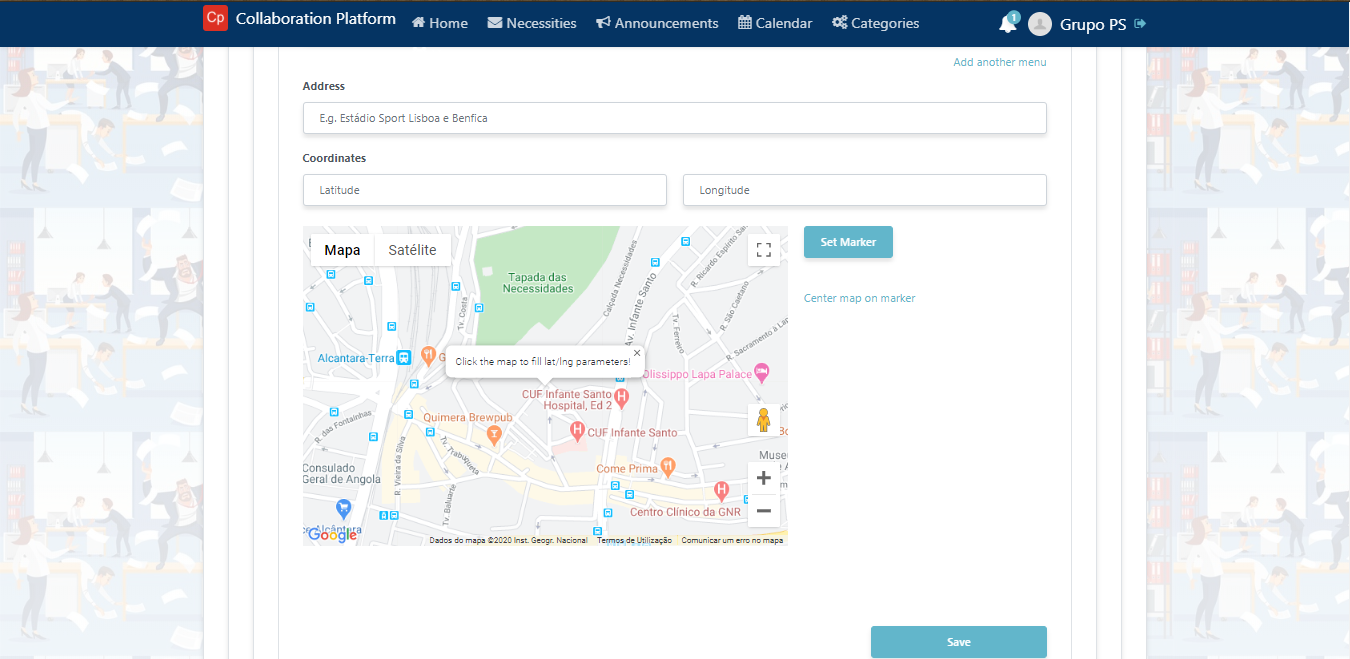
\includegraphics[scale=0.4]{figures/Resources2.png}
  \caption{Ecrã \textit{Necessity Creation} --- Aba de recursos parte 2.}\label{fig:Resources2}
\end{figure}


Na última tab do \textit{widget Accordion} presente no ecrã \textit{NecessityCreation} (figura~\ref{fig:participants}) encontra-se a secção relacionada com os participantes à necessidade. 
Nesta secção um utilizador poderá candidatar-se à posição de colaborador ou participante, de acordo com a fase em que a necessidade se encontra, carregando no \textit{widget link} com o texto \textit{Apply as a Colaborator/Partipant} e deixando uma descrição se a filtragem dos candidatos estiver ativa para aquela necessidade.
Um utilizador, ao criar uma necessidade, tem a opção de escolher se todas as candidaturas são aceites ou se o próprio irá proceder à sua filtragem selecionando um dos \textit{widgets radio button}.  

\begin{figure}[H]
  \centering 
  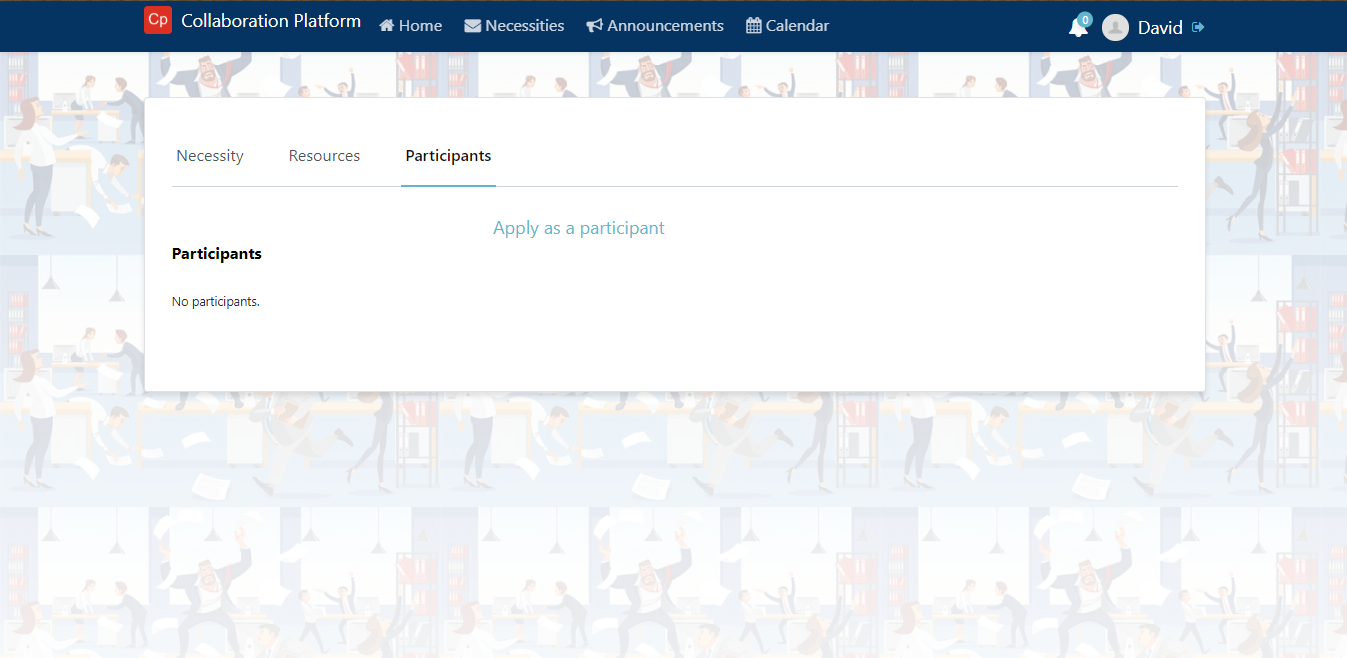
\includegraphics[scale=0.4]{figures/Participants.png}
  \caption{Ecrã \textit{Necessity Creation} --- Aba dos participantes.}\label{fig:participants}
\end{figure}

\subsection{Notificações na plataforma}\label{subsec:implementacao:notificacoes}

A plataforma tem um sistema de notificações que suporta o seu envio para os utilizadores, num ecrã (figura~\ref{fig:notifications}) onde é possível visualizá-las em detalhe. 
Os cenários possíveis de envio de notificações consistem em: sempre que existir uma nova candidatura a uma dada necessidade o autor da mesma é notificado; 
quando um utilizador vê a sua candidatura aceite ou não; 
quando uma necessidade é eliminada ou editada, os participantes da mesma são notificados;
quando um dado utilizador quer desistir da sua participação a uma necessidade, o autor da mesma recebe uma notificação para remover esse participante;
quando uma mensagem enviada para os administradores da plataforma foi resolvida ou rejeitada;
e, por último, quando é o dia em que uma necessidade se vai realizar e a mesma tem \textit{QR code} associado, os participantes recebem uma notificação com um link para o \textit{QR code} gerado.
A cada notificação está associado o \textit{id} do utilizador, o que permite que quando o mesmo navegue até ao ecrã das notificações, 
lhe sejam apresentadas todas as suas notificações que recebeu, provenientes do registo na base de dados.

\begin{figure}[H]
  \centering 
  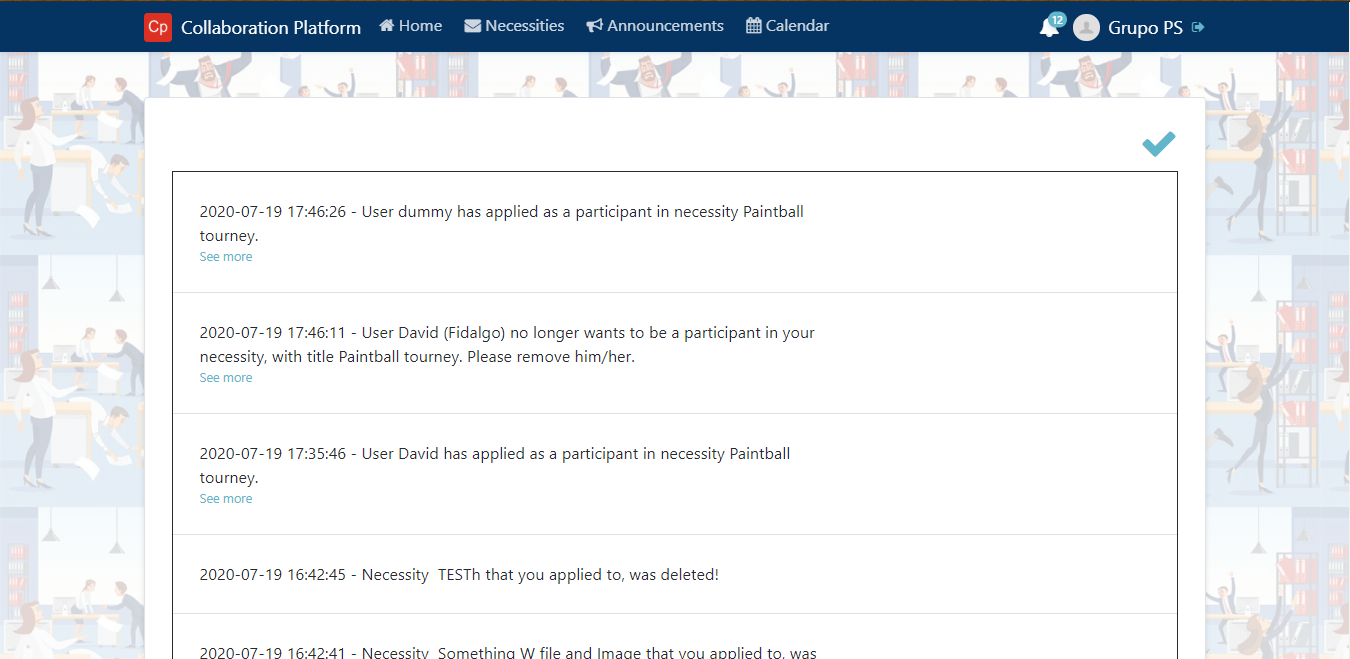
\includegraphics[scale=0.4]{figures/Notifications.png}
  \caption{Ecrã \textit{Notifications} onde cada utilizador pode consultar as suas notificações.}\label{fig:notifications}
\end{figure}

\chapter{Conclusão}\label{sec:conclusion}

De uma forma geral, o progresso do projeto está de acordo com o planeamento apresentado anteriormente, na proposta de projeto, e novamente, na figura~\ref{fig:timeline}.

Inicialmente, devido à pesquisa e aprendizagem de algumas tecnologias novas, o desenvolvimento ocorreu de forma mais lenta. 
No entanto, após ultrapassado esse obstáculo, o ritmo de trabalho aumentou de forma considerável e consequentemente os resultados surgiram também mais rapidamente. 

De momento, a aplicação já possui um modelo de dados estruturado e algumas funcionalidades, nomeadamente a possibilidade de criação, 
inscrição e visualização de uma necessidade, e um \textit{back office} que permite adicionar e/ou remover categorias possíveis de uma necessidade. 
Para além disto, foi desenvolvida uma outra funcionalidade que estava no planeamento ser realizada no próximo sprint, nomeadamente a visualização das necessidades dispostas num calendário.

\begin{figure}[H]
  \centering 
  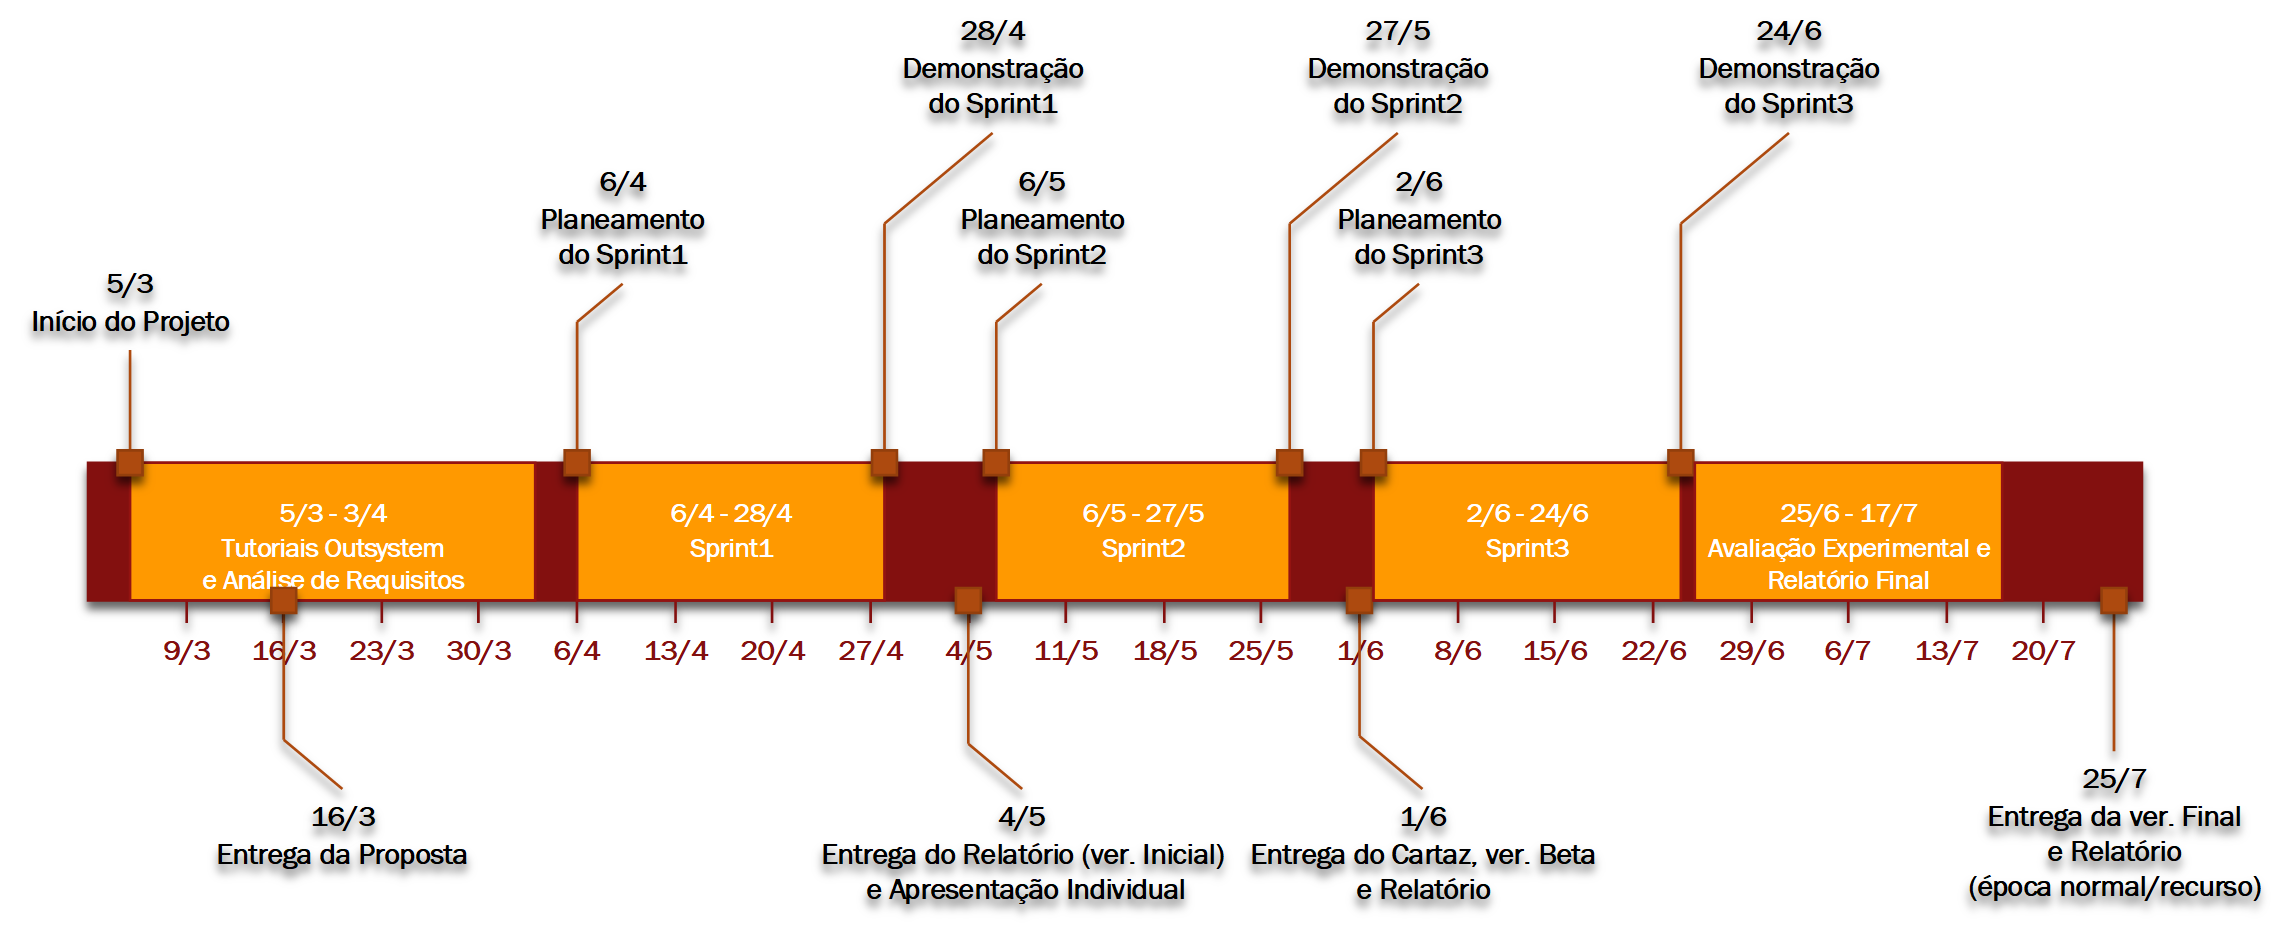
\includegraphics[scale=0.5]{figures/Timeline.png}
  \caption{Timeline}\label{fig:timeline}
\end{figure}

% Referencias

\begin{thebibliography}{9}
  \bibitem{outsystems}
  \href{http://www.outsystems.com}{\textit{OutSystems}}
  
  \bibitem{google maps api}
  \href{https://developers.google.com/maps/documentation/javascript/reference}{Documentação da \textit{API Google Maps}}
  
  \bibitem{places api}
  \href{https://developers.google.com/places/web-service/intro}{Documentação da \textit{API Places}}

  \bibitem{fullcalendar}
  \href{https://fullcalendar.io/docs}{Documentação do componente da \textit{Forge FullCalendar Reactive}}
\end{thebibliography}


\addcontentsline{toc}{chapter}{A.1 Modelo Entidade-Associação da aplicação}
\chapter*{A.1 Modelo Entidade-Associação da aplicação}
\begin{figure}[H]
  \centering 
  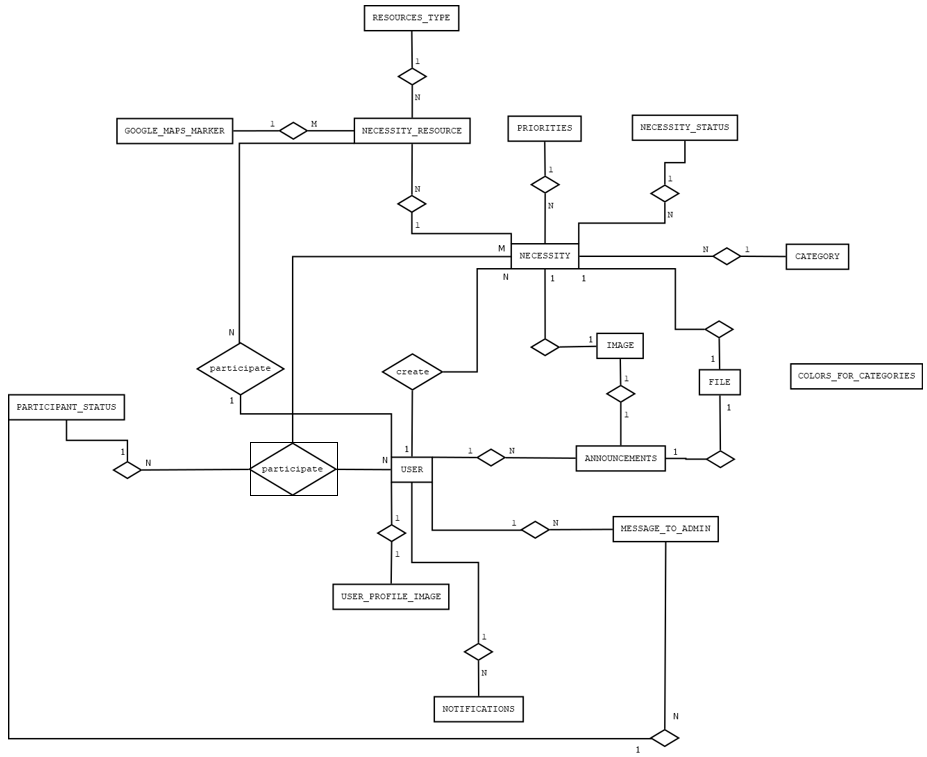
\includegraphics[angle=-90,origin=c, scale=0.6]{figures/ModeloEA.png}
  \caption{Modelo EA}\label{anexo:modeloEA}
\end{figure}


\end{document}